\documentclass[xcolor={x11names,svgnames}]{beamer}
\setbeamerfont{note page}{size=\tiny} % default = small 

%\includeonlyframes{radix,radix_code,radix_noconflict}
%\includeonlyframes{lock-free-defs,seq_intset,lf_intset}


\usecolortheme{rose}
\setbeamertemplate{footline}{}
\setbeamertemplate{navigation symbols}{\footnotesize\insertframenumber}
  
\usepackage{amsmath, amssymb, amsthm}

\usepackage[utf8]{inputenc}
\usepackage[francais]{babel}
\usepackage[T1]{fontenc}
\usepackage[normalem]{ulem}   
%\usepackage{mdframed}
%\usepackage{cancel}
\usepackage{multirow}

\usepackage{minted}
\setminted{fontsize=\scriptsize}

\usepackage{tikz}
\usetikzlibrary{calc}
%\usetikzlibrary{decorations}
%\usetikzlibrary{positioning}
\usetikzlibrary{decorations.pathmorphing}
%\usetikzlibrary{decorations.pathreplacing}
%\usetikzlibrary{shapes.multipart}

\usepackage{fontspec}

\setsansfont{PalatinoSansLTPro}[
   Path = /home/charles/charles_work/fonts/PalatinoSans/, 
   Extension      = .otf,
   UprightFont    = *-Regular,
   BoldFont= *-Bold ,
   ItalicFont = *-Italic,
   BoldItalicFont = *-BoldIta
]

\newcommand{\blue}[1]{{\color{Blue}#1}}
\newcommand{\green}[1]{{\color{LimeGreen}#1}}
\newcommand{\red}[1]{{\color{red}#1}}
\newcommand{\tikzmat}[2] {
\draw[thick] let \p1 = (#1 |- #2),
                 \p2 = (#2 |- #1) in
   ($ (#1) + (0.05,-0.1) $) -- ++(-0.15, 0)  -- ($ (\p1) + (-0.1,0.1) $) -- ++(0.15,0)
   ($ (\p2) + (-0.05,-0.1) $) -- ++(0.15, 0) -- ($ (#2) + (0.1,0.1) $) -- ++(-0.15,0);
}


\author[C.~Bouillaguet]{Charles Bouillaguet \newline
  {\small \texttt{charles.bouillaguet@lip6.fr}}}

\title{Cours 7 : la \og vectorisation\fg}
\date{2020-04-16}


\begin{document}

\frame{\titlepage}

\section{Intro}

\begin{frame}
  \frametitle{Principe}

  \begin{block}{La vectorisation, c'est...}
    \begin{itemize}
    \item Reformuler les algorithmes
    \item pour qu'ils fassent des opérations sur des \textbf{vecteurs}
    \end{itemize}
     
  \end{block}

  \begin{align*}
    A &\gets \lambda B + \mu C & A[i] &\gets \lambda B[i] + \mu C[i]\\
    A &\gets B + C \times D    & A[i] &\gets B[i] + C[i] \times D[i] & (\textit{Fused Multiply-Add}) \\
    A &\gets |B|               & A[i] &\gets |B[i]|  \\
    A &\gets \max(B, C)        & A[i] &\gets \max(B[i], C[i])  \\
    A[B] &\gets C              & A[B[i]] &\gets C[i] & (\textit{scatter}) \\
    A &\gets C[B]              & A[i] &\gets C[B[i]] & (\textit{gather}) \\
    A &\gets B \leq C          & A[i] &\gets B[i] \leq C[i]  \\
  \end{align*}

\end{frame}

%%%%%%%%%%%%%%%%%%%%%%%%%%%%%%%%%%%%%%%%%%%%%%%%%%

\begin{frame}
  \frametitle{Pourquoi ?}

  \begin{block}{Les ops. sur les vecteurs sont \alert{intrinsèquement parallèles}}
    \begin{itemize}
    \item Permet d'exprimer du parallélisme
      \begin{itemize}
      \item Fortran ($\geq 90$), \texttt{numpy} gèrent des vecteurs nativement
      \item Mais pas le C...
      \end{itemize}

      \medskip
      
    \item Il a existé des \alert{processeurs vectoriels}
      \begin{itemize}
      \item Cray 1 (1975)
      \item Cray X-MP (1982)
      \item Cray 2 (1985)
      \item IBM 3090 (1985)
      \item Fujitsu VP2000 (1988)
      \item NEC SX (1992)
      \item ...
      \end{itemize}
    \end{itemize}
  \end{block}
\end{frame}

%%%%%%%%%%%%%%%%%%%%%%%%%%%%%%%%%%%%%%%%%%%%%%%

\begin{frame}
  \frametitle{IBM 3090 CPU}

  \centering
  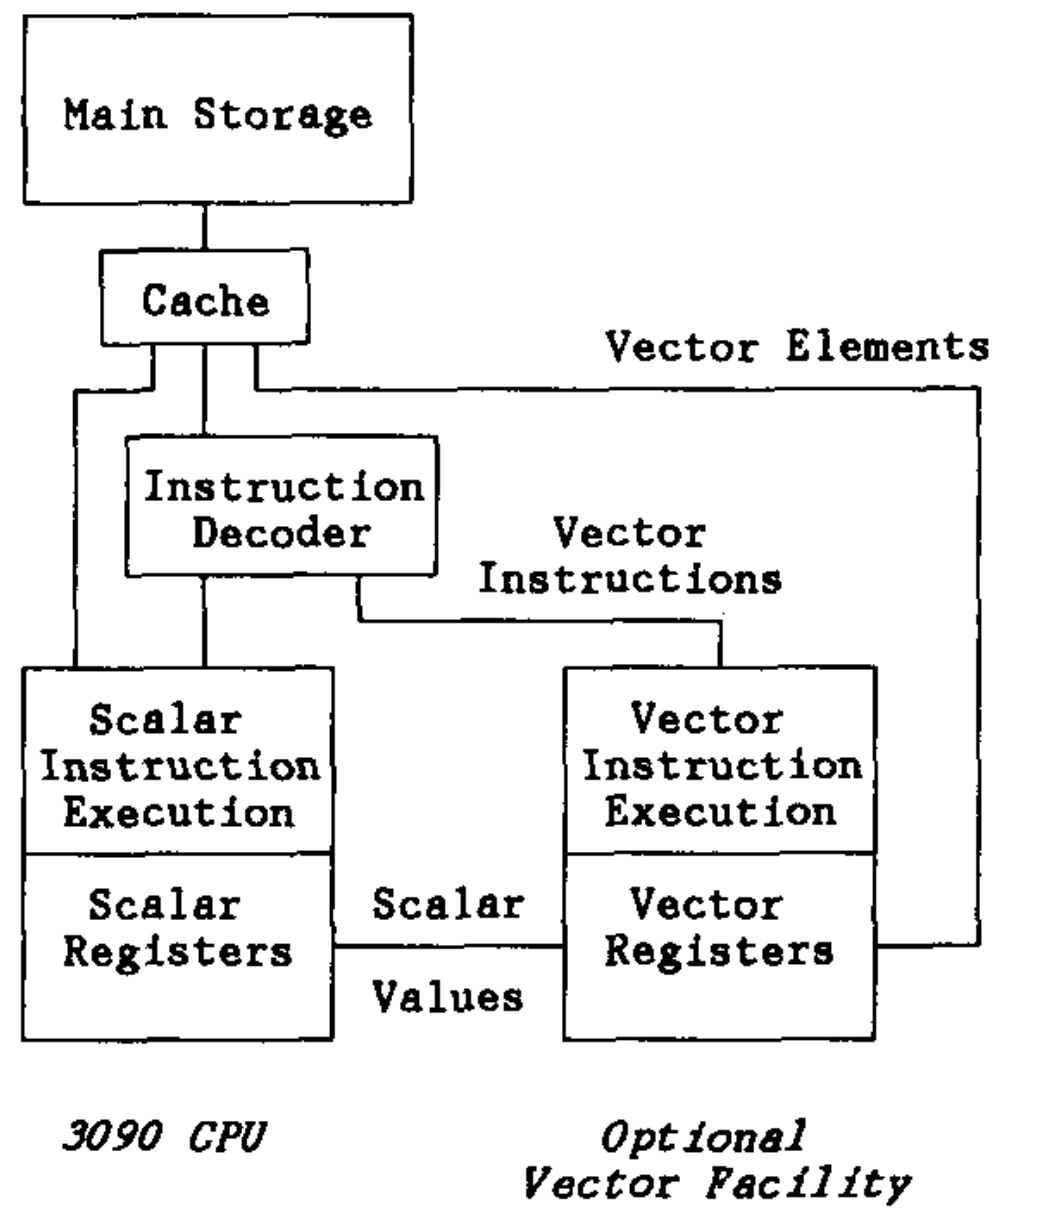
\includegraphics[height=8cm]{ibm_3090.jpg}  
\end{frame}

%%%%%%%%%%%%%%%%%%%%%%%%%%%%%%%%%%%%%%%%%%%%%%

\begin{frame}
  \frametitle{Intérêt des \red{instructions vectorielles}}
  
  \begin{itemize}
  \item Possibilité de traitement parallèle
    \begin{itemize}
    \item bas-de-gamme = un peu
    \item haut-de-gamme = beaucoup
    \end{itemize}

    \medskip
    
  \item Une seule instruction donne beaucoup de travail
    \begin{itemize}
    \item Économies sur le décodage des instructions
    \end{itemize}

    \medskip

  \item Opérations enchainées $\leadsto$ pipelining
    \begin{itemize}
    \item Efficacité énergétique
    \end{itemize}
  \end{itemize}

  \begin{alertblock}{Mais pourquoi ça a disparu ?}
    \begin{itemize}
    \item Nécessite \textbf{mémoire rapide} pour transférer les vecteurs
    \item Scatter/gather sont particulièrement horribles
    \item[$\Rightarrow$] processeurs/machines \emph{dédiés} au HPC
    \item Mais tendance \og \textit{commodity components}\fg{} (ASCI red)
    \end{itemize}
  \end{alertblock}  
\end{frame}

%%%%%%%%%%%%%%%%%%%%%%%%%%%%%%%%%%%%%%%%%%%%%%

\section{Description du hardware}


\begin{frame}
  \frametitle{Le présent : instructions SIMD}

  \begin{enumerate}
  \item[1985] IBM 3090, registres vectoriels de $32 Z$ bits
    \begin{itemize}
    \item $Z$ \alert{pas spécifié}, \textit{implementation-dependent}
    \item Dans les faits, $Z=128$, donc vecteurs de 4096 bits
    \end{itemize}
  \end{enumerate}

  \medskip
    \begin{overlayarea}{\textwidth}{6cm}
    \only<2>{\centering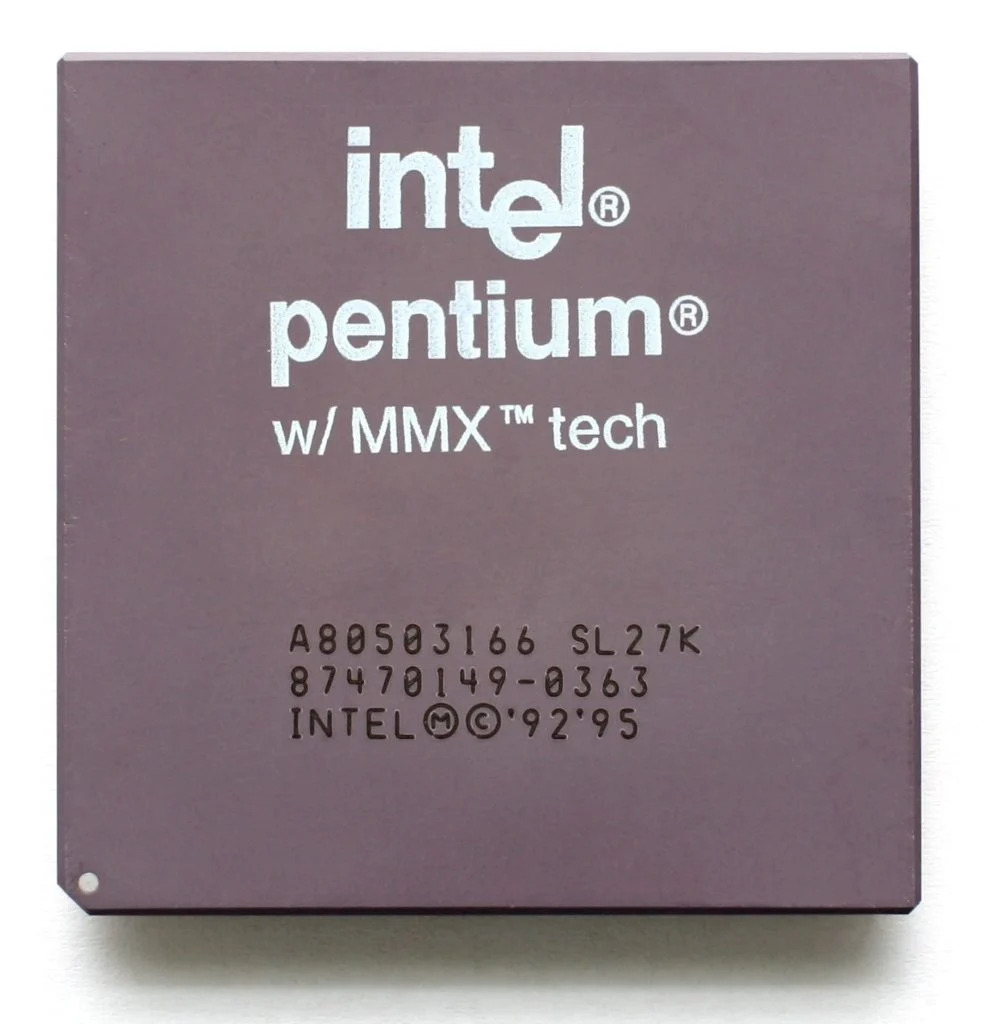
\includegraphics[height=6cm]{pentium_mmx}}
    \pause
    \pause

    \begin{enumerate}  
    \item[1996] Intel Pentium MMX : vecteurs de 64 bits (\texttt{8*int8/4*int16})
      \pause
    \item[1999] Intel SSE : vecteurs de 128 bits, \texttt{4*float}
    \item[2001] Intel SSE2 : vecteurs de 128 bits, \texttt{int} et \texttt{double}
    \item[2004] Intel SSE3 : plus d'opérations
    \item[2007] Intel SSE4 : plus d'opérations
    \item[2010] Intel AVX : vecteurs de 256 bits, \texttt{8*float}
    \item[2010] Intel AVX2 : vecteurs de 256 bits, \texttt{int} et \texttt{double} + \texttt{gather}
    \item[2017] Intel AVX512 : 512 bits, tous types + \texttt{scatter/gather/mask}
  \end{enumerate}
\end{overlayarea}

\end{frame}

%%%%%%%%%%%%%%%%%%%%%%%%%%%%%%%%%%%%%%%%%%%%%%%%

\begin{frame}
  \scriptsize
  \begin{tabular}{|c||c|c|c|c|c|}
  \hline
  ISA & Accronyme & Nom & année & \# regs & |regs| \\
  \hline  \hline
    IBM 3090 & & Vector Facility & 1985 & 16 & variable \\ 
    \hline  \hline
  \multirow{9}{*}{x86-64} & MMX & Multi Media eXtensions & 1996 & 8 & 64 \\
  \cline{2-6}
  & 3DNow! &                                            & 1998 & 8  &  64 \\
    \cline{2-6}
  & SSE    & \multirow{4}{*}{Streaming SIMD Extensions} & 1999 & \multirow{5}{*}{16} & \multirow{5}{*}{128} \\
%    \cline{2-2}
  & SSE2   &                           & 2001 &         & \\
 %   \cline{2-2}
  & SSE3   &                           & 2004 &         & \\
%    \cline{2-2}
  & SSSE3  &                           & 2004 &         & \\
%    \cline{2-2}
  & SSE4   &                           & 2007 &         & \\
    \cline{2-6}
  & AVX    & \multirow{3}{*}{Advanced Vector eXtensions} & 2010 & \multirow{2}{*}{16} & \multirow{2}{*}{256} \\
%    \cline{2-2}
  & AVX2   &                           & 2013  &    &     \\
    \cline{2-2}\cline{4-6}
  & AVX512 &                           & 2017  & 32 & 512 \\
  \hline\hline
  PowerPC & Altivec & & 1999 & 32 & 128 \\
  \hline\hline
  ARM v7 & \multirow{2}{*}{NEON} & \multirow{2}{*}{Advanced SIMD extension}    & 2005 & 16 & \multirow{2}{*}{128} \\
  \cline{1-1}%\cline{4-5}
  \multirow{2}{*}{ARM v8} &      &                            & 2011 & 32 &  \\
  \cline{2-6}
   & SVE  & Scalable Vector Extensions & 2020 & 32 & variable \\
  \hline
\end{tabular}  

\bigskip

\normalsize
\begin{itemize}
\item ARMv8 SVE : registres de 128--2048 bits
\item \texttt{fugaku} implante SVE avec des registres des 512 bits
\item \texttt{RISC-V} a une extension vectorielle inspirée d'IBM 3090
\end{itemize}
\end{frame}

%%%%%%%%%%%%%%%%%%%%%%%%%%%%%%%%%%%%%%%%%%%%%%%%%%%%%%%%%%%%%%%%%%%%%%%%%%%%%%

\begin{frame}
  \frametitle{Deux styles}

\begin{exampleblock}{\og Vraies\fg{} architectures vectorielles à l'ancienne}
  \begin{itemize}
  \item Taille des registres inconnue, voire pas de registres du tout
  \item Fonctionnalités : Scatter + Gather + masques
  \item \textbf{\alert{Revival}}: ARMv8 SVE, RISC-V, AVX-512, ...
  \end{itemize}
\end{exampleblock}

\begin{alertblock}{Instructions SIMD disponibles dans les CPU grand public}
  \begin{itemize}
  \item Taille des registres fixée
  \item Empilement de générations successives
  \item Accès à la mémoire contraint
  \end{itemize}
\end{alertblock}

Entre les deux/à côté : les GPUs
\end{frame}

%%%%%%%%%%%%%%%%%%%%%%%%%%%%%%%%%%%%%%%%%%%%%%%%%%%%%%%%%%%%%%%%%%%%%%%%%%%%%%%

\begin{frame}
  \begin{itemize}
  \item ARM Neon est dans tous les smartphones

    \medskip
    
    \item Presque tous les CPUs x86 ont AVX2 aujourd'hui

      \medskip

    \item AVX512 : pas pour tout le monde
      \begin{itemize}
      \item Xeon bronze/silver/gold depuis 2017
      \item Certains core i3/i5/i7 très récents (mais pas tous...) 
      \end{itemize}
    

    \medskip

  \item Ici : \texttt{ppti-gpu-[1,2,4]} ont l'AVX512
  \item Grid'5000 : certains clusters l'ont
  \end{itemize}
\end{frame}

%%%%%%%%%%%%%%%%%%%%%%%%%%%%%%%%%%%%%%%%%%%%%%%%%%%%%%%%%%%%%% 

\begin{frame}[fragile]

\verb|bouillaguet@ppti-gpu-1:~$ cat /proc/cpuinfo|

\ttfamily\scriptsize
...

\verb|model name        : Intel(R) Xeon(R) Gold 6152 CPU @ 2.10GHz|

...

\verb|flags             :| fpu vme de pse tsc msr pae mce cx8 apic sep mtrr pge mca cmov pat pse36 clflush dts acpi \alert{mmx} fxsr \alert{sse sse2} ss ht tm pbe syscall nx pdpe1gb rdtscp lm constant\_tsc art arch\_perfmon pebs bts rep\_good nopl xtopology nonstop\_tsc cpuid aperfmperf pni pclmulqdq dtes64 monitor ds\_cpl vmx smx est tm2 \alert{ssse3} sdbg fma cx16 xtpr pdcm pcid dca \alert{sse4\_1 sse4\_2} x2apic movbe popcnt tsc\_deadline\_timer aes xsave \alert{avx} f16c rdrand lahf\_lm abm 3dnowprefetch cpuid\_fault epb cat\_l3 cdp\_l3 invpcid\_single pti intel\_ppin ssbd mba ibrs ibpb stibp tpr\_shadow vnmi flexpriority ept vpid ept\_ad fsgsbase tsc\_adjust bmi1 hle \alert{avx2} smep bmi2 erms invpcid rtm cqm mpx rdt\_a \alert{avx512f avx512dq} rdseed adx smap clflushopt clwb intel\_pt \alert{avx512cd avx512bw avx512vl} xsaveopt xsavec xgetbv1 xsaves cqm\_llc cqm\_occup\_llc cqm\_mbm\_total cqm\_mbm\_local dtherm ida arat pln pts pku ospke flush\_l1d
\end{frame}

%%%%%%%%%%%%%%%%%%%%%%%%%%%%%%%%%%%%%%%%%%%%%%%%%%%%%%%%%%%%%%%%

\begin{frame}
  \frametitle{Problèmes avec les jeux d'instructions SIMD}

  Leur multiplicité les rend difficiles à utiliser

  \bigskip
  
  \begin{itemize}
  \item Nécessite recompilation à chaque nouvelle version
    \begin{itemize}
    \item Voire réécriture du code / changement des algos... 
    \end{itemize}

    \medskip
    
  \item Rend le code non-portable
    \begin{itemize}
    \item Le CPU qui va exécuter le programme a-t-il AVX-xxx ? 
    \item Déterminer \alert{à l'exécution} le CPU...
    \item ... Et utiliser la fonction appropriée (soupir)
    \end{itemize}
    
  \end{itemize}
\end{frame}

%%%%%%%%%%%%%%%%%%%%%%%%%%%%%%%%%%%%%%%%%%%%%%%%%%%%%%%%%%%%%%%%%


%%%%%%%%%%%%%%%%%%%%%%%%%%%%%%%%%%% 


\begin{frame}
  \frametitle{SSEx + AVX + AVX2}
  \begin{center}

  \begin{tikzpicture}[xscale=0.3, yscale=0.4, every node/.style={font=\small}]
  \foreach \i in {0, 8, 16, 24}
    \filldraw[thick, fill=orange, fill opacity=0.5] (\i, 0) rectangle +(7.8, 1);

  \foreach \i in {0, 4, ..., 31}
    \filldraw[thick, fill=yellow, fill opacity=0.5] (\i, 1.2) rectangle +(3.8, 1);

  \foreach \i in {0, 16}
    \filldraw[thick, fill=gray, fill opacity=0.5] (\i, 3) rectangle +(15.8, 1);

  \foreach \i in {0, 8, ..., 31}
    \filldraw[thick, fill=gray, fill opacity=0.5] (\i, 4.2) rectangle +(7.8, 1);

  \foreach \i in {0, 4, ..., 31}
    \filldraw[thick, fill=gray, fill opacity=0.5] (\i, 5.4) rectangle +(3.8, 1);

  \foreach \i in {0, 2, ...,  31}
    \filldraw[thick, fill=gray, fill opacity=0.5] (\i, 6.6) rectangle +(1.8, 1);

  \foreach \i in {0, 1, ...,  31}
    \filldraw[thick, fill=gray, fill opacity=0.5] (\i, 7.8) rectangle +(0.8, 1);

    \foreach \i in {0, 8, ..., 31}
    \path (\i, 0) rectangle node {\texttt{double}} +(7.8, 1);

    \foreach \i in {0, 4, ..., 31}
    \path (\i, 1.2) rectangle node {\texttt{float}} +(3.8, 1);

    \foreach \i in {0, 16}
    \path (\i, 3) rectangle node {\texttt{int128}} +(15.8, 1);

    \foreach \i in {0, 8, ..., 31}
    \path (\i, 4.2) rectangle node {\texttt{int64}} +(7.8, 1);

    \foreach \i in {0, 4, ..., 31}
    \path (\i, 5.4) rectangle node {\texttt{int32}} +(3.8, 1);

    \foreach \i in {0, 2, ..., 31}
    \path (\i, 6.6) rectangle  +(1.8, 1);

    \draw[thick,<->] (16, 9.5) -- node[above] {\texttt{\%xmm}$i$} +(15.8, 0);
    \draw[thick,<->] (0, 11) -- node[above] {\texttt{\%ymm}$i$} +(31.8, 0);
  \end{tikzpicture}

  \bigskip
  
\begin{tabular}{|c|c|c|}
  \hline
  Instructions & registres & taille \\
  \hline\hline
  SSE$x$              & \texttt{\%xmm0}, \dots, \texttt{\%xmm15} & 128 bits \\
  \hline
  AVX + AVX2          & \texttt{\%ymm0}, \dots, \texttt{\%ymm15} & 256 bits \\
  \hline
  \multirow{2}{*}{AVX512} & \texttt{\%zmm0}, \dots, \texttt{\%zmm31} & 512 bits \\
               & \texttt{\%k0}, \dots, \texttt{\%k7}      & 64 bits \\
  \hline
  \end{tabular}
\end{center}
\end{frame}

%%%%%%%%%%%%%%%%%%%%%%%%%%%%%%%%%%%

\begin{frame}[fragile=singleslide]
  \frametitle{Nomenclature des instructions}
  
Les instructions SIMD flottantes ont des noms
composés :
\begin{center}
  \verb|<prefix><op><simd or not><type>|
\end{center}
où :
\begin{description}
\item[\texttt{<prefix>}:] vide (SSE), \texttt{v} (AVX, AVX2, AVX512)
\item[\texttt{<op>}] \texttt{add}, \texttt{sub}, \texttt{mul}, \texttt{div}, \texttt{fmadd}, \texttt{min}, \texttt{max}, \texttt{abs}, \texttt{floor}, \texttt{ceil}, \texttt{round}, \dots
\item[\texttt{<simd or not>}] \texttt{s} (\textit{scalar}), \texttt{p} (\textit{packed} --- c.a.d. vecteur).
\item[\texttt{<type>}] \texttt{s} (\textit{single}, \texttt{float}), \texttt{d} (\texttt{double})
\end{description}

\bigskip

E.g. \texttt{vmaxpd}, \texttt{vmulss}, etc.

\end{frame}

%%%%%%%%%%%%%%%%%%%%%%%%%%%%%%%%%%%%%%%%%%%%%%%%%%%%%%%%%%%%%%%%

\section{Principes généraux}

\begin{frame}
  \frametitle{La vectorisation en pratique}

  \begin{block}{Principe général}
    \begin{enumerate}
    \item Charger les données dans registres SIMD
    \item Calculer avec les instructions SIMD
    \item Écrire le résultat en mémoire
    \end{enumerate}
  \end{block}

  (minimiser le nombre de ces transferts est un objectif important)
  
  \begin{alertblock}{Conditions d'utilisation}
    \begin{itemize}
    \item Se déroule à \textbf{l'intérieur d'un thread}
      \begin{itemize}
      \item Parallélisation = répartir sur plusieurs coeurs
      \item Vectorisation = utiliser instructions SIMD dans UN coeur
      \end{itemize}
    \item La vectorisation concerne des \textbf{portions de code réduites}
      \begin{itemize}
      \item \textbf{Boucles} simples (limites du jeu d'instruction) 
      \item [$\Rightarrow$] cible généralement les boucles les \textbf{plus internes}
      \end{itemize}

    \end{itemize}
  \end{alertblock}
\end{frame}  

%%%%%%%%%%%%%%%%%%%%%%%%%%%%%%%%%%%

\begin{frame}[fragile=singleslide]
  \frametitle{Obstacles à la vectorisation}

  \begin{itemize}
  \item Dépendance de donnée (itérations pas indépendantes)
     \begin{minted}{C}
     for (int i = 1; i < n; i++)
         a[i] += a[i-1];
\end{minted}
    \begin{itemize}
    \item Pas de traitement en parallèle possible
      \item[$\hookrightarrow$] Nécessité de changer l'algorithme
    \end{itemize}

\medskip

\item Instructions conditionnelles \texttt{if}
     \begin{minted}{C}
     for (int i = 1; i < n; i++)
         if (a[i] != 0)
             a[i] = 1 / a[i];
\end{minted}
  \begin{itemize}
  \item Éventuellement gérable (avec surcoût --- à éviter si possible)
  \end{itemize}

  \medskip

\item Accès à la mémoire compliqués et/ou pb. d'alignement
  \begin{itemize}
  \item Chargement de portions de tableaux \textbf{contiguës} uniquement 
  \end{itemize}
  
  \medskip

\item Calculs trop compliqués (sin, cos, log, exp, my\_function, ...)
\end{itemize}
\end{frame}  

%%%%%%%%%%%%%%%%%%%%%%%%%%%%%%%%%%%%%%%%%%%%%%

\begin{frame}[fragile=singleslide]
  \frametitle{Problèmes d'alignement}

  \begin{alertblock}{Règle générale}
    Vecteur de $xxx$ octets doit être à une adresse multiple de $xxx$
  \end{alertblock}

  \bigskip
  
  \begin{exampleblock}{Solutions}
    \begin{itemize}
    \item \mintinline{C}{double A[n] __attribute__ ((aligned(32)));}
      \begin{itemize}
      \item Ceci est du code C correct !
      \end{itemize}
  \item \mintinline{C}{int posix_memalign(void **ptr, size_t align, size_t size);}
  \item \mintinline{C}{void *aligned_alloc(size_t alignment, size_t size);}
      \begin{itemize}
      \item Inclus dans le langage C11
      \end{itemize}
  \end{itemize}
\end{exampleblock}
\end{frame}

%%%%%%%%%%%%%%%%%%%%%%%%%%%%%%%%%%%%%%%%%%%%%%

\begin{frame}[fragile=singleslide]
  \frametitle{Problèmes d'accès compliqués à la mémoire}

\begin{alertblock}{Array of struct}
  \begin{minted}{C}
struct point {
      double x, y, z;
};

struct point *A;
  \end{minted}

\texttt{xyzxyzxyzxyzxyzxyz....}
\end{alertblock}

\begin{exampleblock}{Struct of Array}
  \begin{minted}{C}
struct points {
      double *x, *y, *z;
};
struct points A;          // traitement par lot facilité
                          // tableaux d'éléments uniformes
  \end{minted}

  \texttt{xxxxxxxxxxxxxx....}\\
    \texttt{yyyyyyyyyyyyyy....}\\
    \texttt{zzzzzzzzzzzzzz....}\\
\end{exampleblock}

\end{frame}

%%%%%%%%%%%%%%%%%%%%%%%%%%%%%%%%%%%%%%%%%%%

\begin{frame}[fragile=singleslide]
  \frametitle{Vectorisation de boucles simples: \textit{strip-mining}}

  \begin{block}{Code original}
  \begin{minted}{C}
for (int i = 0; i < n; i++)
    u[i] = u[i] + alpha * v[i];
\end{minted}
\end{block}

\begin{exampleblock}{Code transformé}
\begin{minted}{C}
int m = n - (n % 4);
/* traitement par lots de 4 avec instructions SIMD */
for (i = 0; i != m; i += 4) {
    u[i + 0] = u[i + 0] + alpha * v[i + 0];
    u[i + 1] = u[i + 1] + alpha * v[i + 1];
    u[i + 2] = u[i + 2] + alpha * v[i + 2];
    u[i + 3] = u[i + 3] + alpha * v[i + 3];
}
/* épilogue au cas où n ne soit pas un multiple de 4 */
for (int i = m; i < n; i ++)
    u[i] = u[i] + alpha * v[i];
  \end{minted}
\end{exampleblock}
\begin{itemize}
\item Éventuellement : prologue pour l'alignement
\item On peut éviter l'épilogue avec un \textbf{bourrage}
\end{itemize}
\end{frame}

%%%%%%%%%%%%%%%%%%%%%%%%%%%%%%%%%%%%%%%%%%%%%%%%%%%%%%%%%%%%%%%

\begin{frame}[fragile=singleslide]
  \frametitle{Modifications algorithmiques}

  \begin{block}{Point de départ}

\begin{minted}{C}
double sum = 0;
for (int i = 0; i < n; i++)
    sum += a[i];
\end{minted}

    \begin{itemize}
    \item Dépendance de données sur \texttt{sum}
    \end{itemize}
  \end{block}

  \begin{exampleblock}{Code transformé}

\begin{minted}{C}
double __sum[4] = {0, 0, 0, 0};
for (int i = 0; i < n; i += 4) {      // suppose que n est multiple de 4
    __sum[0] += a[i + 0];
    __sum[1] += a[i + 1];
    __sum[2] += a[i + 2];
    __sum[3] += a[i + 3];
}
// épilogue : réduction finale (non-vectorisée)
double sum = __sum[0] + __sum[1] + __sum[2] + __sum[3];
\end{minted}

    \begin{itemize}
    \item Boucle maintenant vectorisable
    \item Léger surcoût dans l'épilogue
    \end{itemize}
  \end{exampleblock}
\end{frame}

%%%%%%%%%%%%%%%%%%%%%%%%%%%%%%%%%%%%%%%%%%%%%%%%%%%%%%%%%%%%%%%%

\section{Comment s'en servir ?}

\begin{frame}
  \frametitle{Comment utiliser les instructions SIMD/vectorielles ?}

  \begin{enumerate}
  \item \sout{Écrire de l'assembleur}

    \medskip
    
  \item Utiliser les \og \textit{instrinsics}\fg{} des compilateurs

\medskip
    
  \item Laisser faire le compilateur (vectorisation automatique)

\medskip
    
  \item Donner des directives de vectorisation (OpenMP $\geq$ v4.0)

    \medskip
    
  \item Utiliser les extensions (non-standard) de \texttt{gcc}

  \end{enumerate}
  
\end{frame}




%%%%%%%%%%%%%%%%%%%%%%%%%%%%%%%%%%%%%%%% 
\subsection{intrinsics}

\begin{frame}[fragile=singleslide]
  \frametitle{Utilisations des \emph{intrinsics}}

  \begin{itemize}
  \item Introduit par Intel, diffusé aux autres compilateurs ensuite
  \item Pseudo-fonctions qui émettent \textbf{une} instruction SIMD
  \item Nécessité de connaître le(s) jeu(x) d'instructions
  \end{itemize}
  
  
\begin{block}{Déclarations}
  \begin{minted}{C}
#include <xmmintrin.h>         // SSE
#include <emmintrin.h>         // SSE2
#include <pmmintrin.h>         // SSE3
#include <tmmintrin.h>         // SSSE3
#include <smmintrin.h>         // SSE4.1
#include <nmmintrin.h>         // SSE4.2
#include <immintrin.h>         // AVX & AVX2 & AVX512
\end{minted}
\end{block}

\end{frame}

%%%%%%%%%%%%%%%%%%%%%%%%%%%%%%%%%%%%%%%%%%%%

\begin{frame}[fragile=singleslide]
  \frametitle{Types de données pour les \emph{intrinsics}}

\begin{block}{Correspondent aux \og vecteurs\fg{} matériels}
  
  \begin{description}
\item[\texttt{\_\_m512}] 512 bits (16 \texttt{float})
\item[\texttt{\_\_m512d}] 512 bits (8 \texttt{double})
\item[\texttt{\_\_m512i}] 512 bits (entiers)

  \item[\texttt{\_\_m256}] 256 bits (8 \texttt{float})
\item[\texttt{\_\_m256d}] 256 bits (4 \texttt{double})
\item[\texttt{\_\_m256i}] 256 bits (entiers)

\item[\texttt{\_\_m128}] 128 bits (4 \texttt{float})
\item[\texttt{\_\_m128d}] 128 bits (2 \texttt{double})
\item[\texttt{\_\_m128i}] 128 bits (entiers)
\end{description}
\end{block}
\end{frame}

%%%%%%%%%%%%%%%%%%%%%%%%%%%%%%%%%%%%%%%%%%%% 

\begin{frame}[fragile=singleslide]
  \frametitle{Exemples}

  \begin{itemize}
  \item \mintinline{C}{_mm256_set1_ps}
  \item \mintinline{C}{_mm256_load_pd}
  \item \mintinline{C}{_mm256_xor_si256}
  \item \mintinline{C}{_mm256_srli_epi32}
  \item \mintinline{C}{_mm256_i32gather_mask_pd}
  \item \mintinline{C}{_mm256_cmpeq_epi32}
  \item \mintinline{C}{_mm256_movemask_epi8}
  \item ...
  \end{itemize}
\end{frame}

%%%%%%%%%%%%%%%%%%%%%%%%%%%%%%%%%%%%%%%%%%%

\begin{frame}[fragile=singleslide]
  \frametitle{Nomenclature générale}

  \begin{center}
    \verb|   _mm_<operation>_<suffix>(param1, param2)        |
    
    \verb|_mm256_<operation>_<suffix>(param1, param2, param3)|

    \verb|_mm512_<operation>_<suffix>(param1, param2, param3)|
  \end{center}

  \begin{block}{\texttt{<suffix>} en deux parties}
    \begin{itemize}
    \item 1ère partie :
      \begin{itemize}
      \item \texttt{p} (packed) et \texttt{ep} (extended packed) : calcul SIMD
      \item \texttt{s} (scalar) : vecteur vu comme 1 seul élément
      \end{itemize}

    
  \item 2ème partie (type)
    \begin{itemize}
    \item{}  [\texttt{s}/\texttt{d}] : nombre flottant en simple ou double précision
    \item{} [\texttt{i}/\texttt{u}]\texttt{nnn} : entier signé ou non-signé (unsigned) de \texttt{nnn} bits (\texttt{nnn} vaut 512, 256, 128, 64, 32, 16, ou 8)
    \end{itemize}
  \end{itemize}
\end{block}
\end{frame}

%%%%%%%%%%%%%%%%%%%%%%%%%%%%%%%%%%%%%%%%%%%%%%

\begin{frame}[fragile=singleslide]
  \frametitle{Exemple}

  \begin{block}{Code original}
\begin{minted}{C}
double alpha;
double u[], v[];
// ...
for (int i = 0; i < n; i++)
    u[i] = u[i] + alpha * v[i];
\end{minted}
\end{block}

\begin{exampleblock}{Code vectorisé (AVX2)}
\begin{minted}{C}
__m256d valpha = _mm256_set1_pd(alpha);   // (alpha, alpha, alpha, alpha)
for (i = 0; i != m; i += 4) {
    /* traitement par lots de 4 */
    __m256d vu = _mm256_load_pd(&u[i]);        // alignement nécessaire
    __m256d vv = _mm256_load_pd(&v[i]);        // alignement nécessaire
    __m256d vres = _mm256_fmadd_pd(valpha, vv, vu);
    _mm256_store_pd(&u[i], vres);              // alignement nécessaire
}
  \end{minted}
\end{exampleblock}
\end{frame}

%%%%%%%%%%%%%%%%%%%%%%%%%%%%%%%%%%%%%%%%%%%%%%%% 

\begin{frame}[fragile=singleslide]
  \frametitle{Exemple : conversions colorimétriques}

  R, G, B, C, M, Y, K = flottant dans $[0; 1]$

  \begin{exampleblock}{Sens facile à vectoriser}
  \[
  \left\{
    \begin{array}{rl}
      R &= (1-C) \times (1 - K) \\
      G &= (1-M) \times (1 - K) \\
      B &= (1-Y) \times (1 - K)
    \end{array}
    \right.
\]
\end{exampleblock}

\begin{alertblock}{Sens problématique}
  \begin{itemize}
  \item Si $(R, G, B) = (0, 0, 0)$ alors $(C,M,Y,K) = (0, 0, 0, 1)$
    
  \item Sinon
    \[  \left\{\begin{array}{rl}
      K &= 1 - \max(R, G, B) \\
      C &= 1 - R  / (1 - K) \\
      M &= 1 - G  / (1 - K) \\
      Y &= 1 - B  / (1 - K) 
    \end{array}
    \right.
\]
\end{itemize}


\end{alertblock}
\end{frame}

%%%%%%%%%%%%%%%%%%%%%%%%%%%%%%%%%%%%%%%%%%%%%%%%%%%%%%%%%%%%%%%%%%%%%%%%%%%%%

\begin{frame}[fragile=singleslide]
  \frametitle{Problèmes d'instructions conditionnelles}
  \framesubtitle{Exemple : RGB $\rightarrow$ CMYK}

  \begin{block}{$K = 1 - \max(R, G, B)$}
\begin{minted}{C}
__m256 vone = _mm256_set1_ps(1.0);            // (1, 1, 1, 1, 1, 1, 1, 1)
// ...
/* traite un chunk de 8 couleurs */
__m256 vR = _mm256_load_ps(&R[i]);               // alignement nécessaire
__m256 vG = _mm256_load_ps(&G[i]);               // alignement nécessaire
__m256 vB = _mm256_load_ps(&B[i]);               // alignement nécessaire
__m256 vmax = _mm256_max_ps(_mm256_max_ps(vR, vG), vB);
__m256 vK = _mm256_sub_ps(vone, vmax);
_mm256_store_ps(&K[i], vk);                      // alignement nécessaire
\end{minted}
\end{block}

  \begin{alertblock}{Si $K < 1$}
\begin{minted}{C}
__m256 vC = _mm256_sub_ps(vone, _mm256_div_ps(vR, vmax));
__m256 vM = _mm256_sub_ps(vone, _mm256_div_ps(vG, vmax));
__m256 vY = _mm256_sub_ps(vone, _mm256_div_ps(vB, vmax));
\end{minted}
  \end{alertblock}  
\end{frame}

%%%%%%%%%%%%%%%%%%%%%%%%%%%%%%%%%%%%%%%%%%%%%%%%%%%%%%%%%%%%%%%%%%%%%%%%%%%

\begin{frame}[fragile=singleslide]
  \frametitle{Problèmes d'instructions conditionnelles}
  \framesubtitle{Exemple : RGB $\rightarrow$ CMYK}

  \begin{exampleblock}{Si $K = 1$}
\begin{minted}{C}
    __m256 vzero = __m256 _mm256_setzero_ps();
    __m256 vmask = _mm256_cmp_ps(vK, vone, _CMP_EQ_OQ);
    // vmask[i] == (vK[i] == 1.0) ? 0xffffffff : 0x00000000 
    vC = _mm256_blendv_ps(vzero, vC, vmask);
    vM = _mm256_blendv_ps(vzero, vM, vmask);
    vY = _mm256_blendv_ps(vzero, vY, vmask);
    // blendv : vX[i] =  vmask[i]       ? vzero[i] : vX[i]
    //                  (vK[i] == 1.0)  ? vzero[i] : vX[i]   
\end{minted}
  \end{exampleblock}

  \begin{block}{Intructions de déplacement au sein des registres}
  \begin{itemize}
  \item \texttt{blend}, \texttt{blendv}, \texttt{broadcast}, \texttt{extract}, \texttt{insert}, \texttt{permute},  \texttt{permutevar}, \texttt{shuffle}, \texttt{unpackhi}, \texttt{unpacklo}, ...
  \end{itemize}
\end{block}
\end{frame}

%%%%%%%%%%%%%%%%%%%%%%%%%%%%%%%%%%%%%%%%%%%%%%%%%%%%%%%%%%%%%%%%%%%%%%

\begin{frame}[fragile=singleslide]
  \frametitle{Problèmes d'instructions conditionnelles}
  \framesubtitle{Exemple : RGB $\rightarrow$ CMYK}

\begin{minted}{C}
__m256 vone, vzero, vmask, vR, vG, vB, vC, vM, vY, vK;
vone = _mm256_set1_ps(1.0);            // (1, 1, 1, 1, 1, 1, 1, 1)
vzero = _mm256_setzero_ps();           // (0, 0, 0, 0, 0, 0, 0, 0)
for (int i = 0; i < n; i += 8) {
    vR = _mm256_load_ps(&R[i]);           // alignement nécessaire 
    vG = _mm256_load_ps(&G[i]);           // alignement nécessaire
    vB = _mm256_load_ps(&B[i]);           // alignement nécessaire
    vmax = _mm256_max_ps(_mm256_max_ps(vR, vG), vB);
    vK = _mm256_sub_ps(vone, vmax);
    vC = _mm256_sub_ps(vone, _mm256_div_ps(vR, vmax));
    vM = _mm256_sub_ps(vone, _mm256_div_ps(vG, vmax));
    vY = _mm256_sub_ps(vone, _mm256_div_ps(vB, vmax));
    vmask = _mm256_cmp_ps(vK, vone, _CMP_EQ_OQ);
    vC = _mm256_blendv_ps(vzero, vC, vmask);
    vM = _mm256_blendv_ps(vzero, vM, vmask);
    vY = _mm256_blendv_ps(vzero, vY, vmask);
    _mm256_store_ps(&C[i], vC);                  // alignement nécessaire
    _mm256_store_ps(&M[i], vM);                  // alignement nécessaire
    _mm256_store_ps(&Y[i], vY);                  // alignement nécessaire
    _mm256_store_ps(&K[i], vK);                  // alignement nécessaire
}
\end{minted}
\end{frame}

\subsection{OpenMP}

%%%%%%%%%%%%%%%%%%%%%%%%%%%%%%%%%%%%%%%%%%%

\begin{frame}[fragile=singleslide]
  \frametitle{Directive OpenMP simd}

  Rappel: nécessite l'option \texttt{-fopenmp}

  \bigskip
  
  \begin{minted}{C}
    #pragma omp simd
    for (int i = 0; i < n; i++)
       ...
  \end{minted}

  \begin{itemize}
  \item Regroupe les itérations en \textit{chunks} de taille $N$
    \begin{itemize}
    \item effectue le calcul avec une unité SIMD à $N$ éléments
    \end{itemize}
    
  \item On \og promet\fg{} au compilateur que la boucle est vectorisable
  \item Pas de parallélisation multi-thread 
  \end{itemize}
\end{frame}

%%%%%%%%%%%%%%%%%%%%%%%%%%%%%%%%%%%%%%%% 

\begin{frame}[fragile=singleslide]
  \frametitle{Directive OpenMP simd}
  
  \begin{minted}{C}
    #pragma omp simd [clause[[,] clause],...]
    for (int i = 0; i < n; i++)
        ...
   \end{minted}

   \begin{block}{Clauses possibles (liste non-exhaustive)}
     \begin{itemize}
     \item \texttt{reduction(+:v}) : déjà connu
       \begin{itemize}
       \item Casse dépendance de données sur la variable qui accumule
       \end{itemize}
       \smallskip
       
     \item \texttt{simdlen(length)}: taille de \textit{chunk} souhaitée
\smallskip
       
     \item \texttt{safelen(length)}: taille de \textit{chunk} maximale
       \begin{itemize}
       \item E.g., au-delà, un problème de dépendance pourrait arriver
       \end{itemize}
\smallskip
       
     \item \texttt{aligned(v[:k])}: promet que $v$ est alignée sur \texttt{k} octets
\smallskip


     \item \texttt{linear(x[:step])}: $x$ dépend de $i$ (\mintinline{C}{x_i = x_init + i * step;})
     \end{itemize}
   \end{block}
 \end{frame}


\subsection{Vectorisation auto}

%%%%%%%%%%%%%%%%%%%%%%%%%%%%%%%%%%%%%%%%%%%%%%%%%%%%%%%%%%%%%%%%%%%%%%%

\begin{frame}[fragile=singleslide]
  \frametitle{Vectorisation automatique}

  \begin{itemize}
  \item Fortran a des vecteurs explicites
    \begin{itemize}
    \item Facile à vectoriser
    \end{itemize}
    \item En C, le compilateur détecte les \textbf{boucles vectorisables}

  \end{itemize}

\begin{exampleblock}{Code C}
\begin{minted}{C}
for (int i = 0; i < n; i++)
        C[i] = lambda * A[i] + mu * B[i];
\end{minted}
\end{exampleblock}

\begin{alertblock}{Code assembleur produit par gcc}

\begin{minted}{gas}
.loop:
        vmulpd  (%rsi,%rax), %ymm3, %ymm0    
        vmulpd  (%rcx,%rax), %ymm2, %ymm1
        vaddpd  %ymm1, %ymm0, %ymm0
        vmovapd %ymm0, (%rdx,%rax)
        addq    $32, %rax
        cmpq    %rcx, %rax
        jne     .loop
\end{minted}
\end{alertblock}%$
\end{frame}


%%%%%%%%%%%%%%%%%%%%%%%%%%%%%%%%%%%%%%%%%%%%%%%%%%%%%%%%%%%%%%%%%

\begin{frame}[fragile=singleslide]
  \frametitle{Instructions SIMD dans le compilateur gcc}

    \begin{itemize}
    \item La \textbf{vectorisation automatique} est désactivée par défaut 
      \begin{itemize}
      \item Par défaut, GCC compile au niveau d'optimisation zéro
      \item Vectorisation automatique et via OpenMP sont désactivées
      \end{itemize}

      \medskip
      
    \item On peut l'activer par l'option \verb|-ftree-vectorize|
      \begin{itemize}
      \item \verb|-O3| entraine cette option
      \end{itemize}
    \item On fait du HPC : compiler avec \verb|-O2| ou \verb|-O3| !
  \begin{minted}{shell}
~$ gcc -O1 -ftree-vectorize vectorisation_auto.c
~$ gcc -O1 -fopenmp vectorisation_omp.c
\end{minted}

\medskip
  
  \item gcc n'émet \textbf{pas} les instructions AVX2 (resp. FMA) par défaut
    \begin{itemize}
    \item Ajouter options \verb|-mavx2| (resp. \verb|-mfma|).
    \end{itemize}

\medskip

\item Verbosité et diagnostic:
  \begin{itemize}
  \item \scriptsize \verb|-fopt-info-vec|, \verb|-fopt-info-vec-missed| et \verb|-fopt-info-vec-all|
  \end{itemize}
  \end{itemize}

  
    % Il n'est très simple de vérifier si les bonnes instructions vectorielles sont utilisées, mais on peut tenter de désassembler le binaire produit à leur recherche. Par exemple, pour vérifier l'utilisation de l'instruction mulps :

    % 		objdump -d ./executable | grep mulps
\end{frame}

%%%%%%%%%%%%%%%%%%%%%%%%%%%%%

\section{FFT}

\begin{frame}
  \frametitle{Étude de cas : la FFT}

  \begin{itemize}
  \item La \textbf{Transformée de Fourier Discrete} (DFT) d'un tableau $X$ de
    $n$ nombres complexes est le tableau $Y$ de taille $n$ défini par
\[
  Y[k] = \sum_{j=0}^{n-1} X[j] \omega_n^{jk}, \qquad \text{avec} \qquad \omega_n = e^{-\frac{2i\pi}{n}}
\]

\medskip

\item Lorsque $n = n_1 \times n_2$, on pose
$j = j_1 n_2 + j_2$ et $k = k_1 + k_2 n_1$ 
\[
Y[k_1 + k_2 n_1] = \sum_{j_2 = 0}^{n_2 - 1} \left[ \left( \sum_{j_1 = 0}^{n_1 - 1} X[j_1n_2 + j_2] {\omega_{n_1}}^{j_1 k_1} \right) {\omega_n}^{j_2 k_1} \right] {\omega_{n_2}}^{j_2 k_2}
\]

\item Omniprésence dans le calcul scientifique
\item Bibliothèques optimisées (e.g. FFTW)
\end{itemize}
\end{frame}

%%%%%%%%%%%%%%%%%%%%%%%%%%%%%%%%%%%%%%%%%%%%%%%%%%%%%%%

\begin{frame}
  \frametitle{FFT : algorithme récursif}

$n = n_1 \times n_2$, on pose $j = j_1 n_2 + j_2$ et $k = k_1 + k_2 n_1$ 

\[
Y[k_1 + k_2 n_1] = \sum_{j_2 = 0}^{n_2 - 1} \left[ \left( \sum_{j_1 = 0}^{n_1 - 1} X[j_1n_2 + j_2] {\omega_{n_1}}^{j_1 k_1} \right) {\omega_n}^{j_2 k_1} \right] {\omega_{n_2}}^{j_2 k_2}
\]
  
\begin{block}{Algorithme pour le calcul de la DFT de taille $n_1 \times n_2$}
  \begin{enumerate}
  \item Calculer $n_2$ DFT de taille $n_1$ (somme interne)
  \item Multiplier par les \emph{twiddle factors} ${\omega_n}^{j_2 k_1}$
  \item Effectuer $n_1$ DFT de taille $n_2$ (somme externe)
  \end{enumerate}
\end{block}

\end{frame}

%%%%%%%%%%%%%%%%%%%%%%%%%%%%%%%%%%%%%%%%%%%%%%%%%%%%%%%%%%%

\begin{frame}[fragile]
  \frametitle{FFT : algorithme récursif}
  \framesubtitle{Présentation classique}

  \begin{itemize}
  \item Choix commun : $n_2 = 2$ (\og \textit{Radix-2 Decimation in Time}\fg).
  \end{itemize}

  \begin{columns}[T]
    \begin{column}{8cm}
      
\begin{minted}{C}
void FFT(const double * X, double *Y, int n, int s)
{
    if (n == 1)
       return;
    double omega_n = exp(-2*I*pi / n);
    double omega = 1;
    FFT(&X[0], &Y[0]  , n/2, 2*s);
    FFT(&X[s], &Y[n/2], n/2, 2*s);
    for (int i = 0; i < n/2; i++) {
        double p = Y[i];
        double q = Y[i + n/2] * omega;
        Y[i] = p + q;
        Y[i + n/2] = p - q;
        omega *= omega_n;    
    }
}
\end{minted}

    \end{column}
    \begin{column}{1.6cm}
    
\begin{tikzpicture}[scale=0.5,line around/.style={decoration={pre length=#1,post length=#1}}]
  \fill[fill=LimeGreen] (0, 0) rectangle (1, 10);
  \fill[fill=cyan] (1, 0) rectangle (2, 10);
  \draw[thick] (0, 0) rectangle (2, 10);

  \draw (1, 0) -- (1, 10);
  \draw[<->] (3, 0) -- node[right] {$\frac{n}{2}$} (3, 10);
  \draw[<->] (0, 11) -- node[above] {$2$} (2, 11);

  % 1ère passe FFT
  \foreach \i in {0.5, 1.5}
    \draw<2>[decorate, decoration=snake, line around=1mm, <->] (\i, 0.1) -- +(0, 9.8);
\end{tikzpicture}
\end{column}
\end{columns}
\end{frame}

%%%%%%%%%%%%%%%%%%%%%%%%%%%%%%%%%%%%%%%%%%%%%%%%%%%%%%%%%%% 

\begin{frame}[fragile]
  \only<1-2>{
  \[
    Y[k_1 + k_2 n_1] = \sum_{j_2 = 0}^{n_2 - 1} \left[ \left( \sum_{j_1 = 0}^{n_1 - 1} X[j_1n_2 + j_2] {\omega_{n_1}}^{j_1 k_1} \right) {\omega_n}^{j_2 k_1} \right] {\omega_{n_2}}^{j_2 k_2}
  \]
}
\only<3>{
  \[
    Y[k_1 + k_2 n_1] = \sum_{j_2 = 0}^{n_2 - 1} \left( U[k_1 n_2 + j_2] {\omega_n}^{j_2 k_1} \right) {\omega_{n_2}}^{j_2 k_2}
  \]
}
\only<4>{
  \[
    Y[k_1 + k_2 n_1] = \sum_{j_2 = 0}^{n_2 - 1} V[k_1 n_2 + j_2] {\omega_{n_2}}^{j_2 k_2}
  \]
}

\begin{itemize}
\item<2-> $U[\star, j_2] \gets FFT(X[\star, j_2])$ (pour tout $0 \leq j_2 < n_2$)
\item<3-> $V[k_1, j_2] \gets U[k_1, j_2] \cdot {\omega_n}^{j_2 k_1}$ (pour tout $0 \leq j_2 < n_2$ et $0 \leq k_1 < n_1$)
\item<4-> $Y[k_1, \star] \gets FFT(U[k_1, \star])$ (pour tout $0 \leq k_1 < n_1$)
\end{itemize}


\begin{tikzpicture}[scale=0.5,line around/.style={decoration={pre length=#1,post length=#1}}]
  \filldraw[thick, fill=LimeGreen] (0, 0) rectangle (16, 9);
  %\foreach \i in {1, 2, ..., 8}
  %\draw (0, \i) -- (16, \i);

  \foreach \i in {1, 2, ..., 15}
  \draw<2> (\i, 0) -- (\i, 9);

  \draw[<->] (17, 0) -- node[right] {$n_1$} (17, 9);
  \draw[<->] (0, 10) -- node[above] {$n_2$} (16, 10);

  % 1ère passe FFT
  \foreach \i in {0, 1, 2, ..., 15} {
    \draw<2>[decorate,decoration=snake, line around=1mm,<->] (\i + 0.5, 0.1) -- +(0, 8.8);
  }

  % pointeurs k_1, j2 dans la première passe
  \draw<2>[->] (-1, 4) node[left] {$k_1$} -- (-0.1, 4); 
  \draw[->] (12.5, -1) node[below] {$j_2$} -- (12.5, -0.1); 

  % twiddle
  \foreach \i in {0.5, 1.5, ..., 15.5} {
    \foreach \j in {0.5, 1.5, ..., 8.5} {
      \draw<3>[black,variable=\t,smooth,domain=0:21.20,samples=20] (\i, \j) plot ({\i + 0.0225 * \t *sin(\t r)}, {\j + 0.0225 * \t * cos(\t r)});
    }
  }
  
  
\end{tikzpicture}

\end{frame}
\end{document}


%%% Local Variables:
%%% TeX-command-extra-options: "-shell-escape"
%%% TeX-engine: xetex
%%% ispell-local-dictionary: "french"
%%% eval: (flyspell-mode 1)
%%% eval: (reftex-mode 1)
%%% End:
